% Drawing 136/13-1 -- folder 136, batch 13, archive page 252 (PDF page 253).
% Transcription: petit croquis d'un triangle (ou tétraèdre) traversé de segments
% Kind: small triangle (or tetrahedron) crossed by segments. Method 2 (schematic redraw from the facsimile). Status: ok.
% Notes: Four points joined like a tetrahedron seen from the side: two triangles A-D-C and A-B-C sharing the doubled edge A-C, and a segment from D to B crossing it; a short stroke beyond D.
% Coordinates: 1 unit = 1 mm = 1/100 of the crop width (bbox in page fractions: [0.71, 0.66, 0.8, 0.72]).
% Redrawn by Claude (claude-opus-5-5), issue #73, 2026-11-07; not checked by a human; not compiled (no TeX in the session).
% Rights: reproduces part of the work -- behind RENDER_TRANSCRIPTS, never published by itself.
\documentclass[tikz,border=3pt]{standalone}
\usepackage{amsmath,amssymb}
\usetikzlibrary{patterns,arrows.meta}
\tikzset{pencil/.style={black!45}, struck/.style={black!35}, mark/.style={circle,draw,inner sep=1.3pt}, pt/.style={circle,fill,inner sep=0.9pt}, opt/.style={circle,draw,fill=white,inner sep=1.1pt}}
\begin{document}
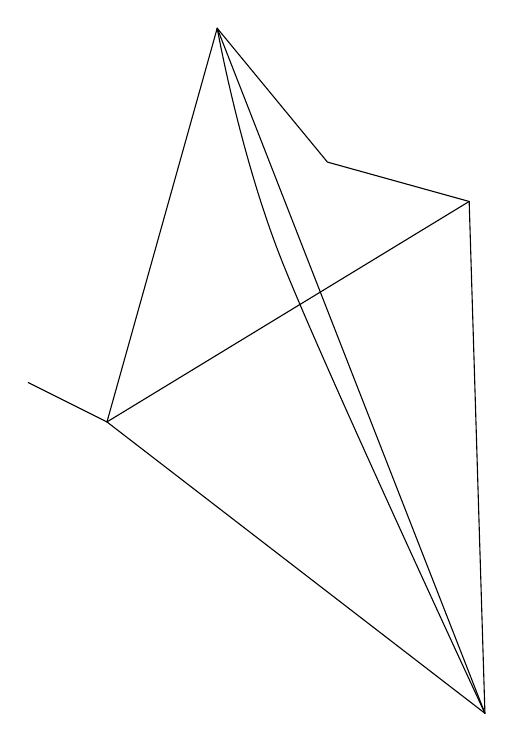
\begin{tikzpicture}[x=1mm,y=1mm,line cap=round,line join=round,font=\scriptsize]
\draw (44,-11) -- (30,-61);
\draw (30,-61) -- (78,-98);
\draw (44,-11) -- (78,-98);
\draw plot[smooth, tension=0.55] coordinates {(44,-11) (52,-40) (78,-98)};
\draw (44,-11) -- (58,-28) -- (76,-33);
\draw (76,-33) -- (78,-98);
\draw (30,-61) -- (76,-33);
\draw (20,-56) -- (30,-61);
\end{tikzpicture}
\end{document}
